\documentclass[times, utf8, seminar]{fer}
\usepackage{booktabs}
\usepackage{epigraph}
\usepackage{mathtools, amsmath,amsfonts,amssymb, amsthm}
\usepackage{hyperref}

\usepackage{etoolbox}
\makeatletter
\patchcmd{\chapter}{\if@openright\cleardoublepage\else\clearpage\fi}{}{}{}
\makeatother

\begin{document}
\theoremstyle{definition}
\newtheorem{definition}{Definition}[section]

\title{Određivanje 5-faktorskog modela ličnosti}
\author{Neven Miculinić}

\maketitle
\tableofcontents

\chapter{Opis problema}

\epigraph{Imagine for yourself a character, a model personality, whose example you determine to follow, in private as well as in public.
}{\textit{Epictetus}}
Ličnost jedan je od temeljnih pojmova psihologije koji se odnosi na neponovljiv, relativno čvrsto integriran, stabilan i kompleksan psihički sklop osobina, koji određuje karakteristično i dosljedno ponašanje individue.-\textit{Wikipedia}.
Kao takva oblikuje naše ponašanje, razmišljanja i stavove; pomaze nam modelirati događaje kako na mikro, tako i na makro razini. Utjecaj ličnosti je primjecen u e-mail adresama~\cite{mail-personality}, sobama i radnim okolinama~\cite{gosling2002room}, interpersonalnim odnosima te mnogim drugim domenama.
No opisati i kategorizirati osobnost nije lak zadatak, te on zalazi u domenu eksperta --- psihologa.
Budući da su oni relativno rijetki i sam čin prikupljanja dojmova može biti dugotrajan i skupocjen postupak razvijeni su ekspertni sustavi --- psihometrijski testovi~\cite{cronbach1949essentials} koji nam pomažu doći do odgovora.
\chapter{5-faktorski model}

Pet faktorski model~\cite{mccrae1992introduction} je danas de facto standardni model ličnosti korišten u svim relevantnim istraživanjima.
Razvijen na temelju statističkog i leksičkog pristupa, 1961.~\cite{tupes1961recurrent} godine.
Leksički model ličnosti se temelji na leksičkoj hipotezi --- sve bitne osobine pojedinca ukodirana su u našem jeziku.
Skupljanjem svih opisnih rijeci osobnosti (vrijedan, pouzdan, otvoren, \ldots) te provođenjem faktorske analize (statistički pristup) dobivamo pet faktora osobnosti.
Tih pet faktora su pronađeni u repliciranim istraživanjima nad raznim jezicima, kulturama i unutar oba spola.
Razvijeni su i slični modeli na životinjama~\cite{king1997five}. Tih pet faktora su:

\begin{itemize}
    \item \textbf{Otvorenost}
    \item \textbf{Savijesnost}
    \item \textbf{Ekstraverzija}
    \item \textbf{Ugodnost}
    \item \textbf{Neuroticizam}
\end{itemize}

Za potrebe ovoga projekta korišten je standardni 44 čestica(pitanja) dug ``Big five inventory''~\cite{john1999big}.

\chapter{Opis alata}
Alat je implementiran kao sustav s pravilima.
Izrađen je u python3 s Flask web serverom, YAML konfiguracijskom datotekom (voluptuous za validaciju istoga), te podatke sprema u SQL bazu pomoću SQLAlchemy biblioteke.

Za izradu na web sučelju rabi Dash biblioteku od Plotly.
Ona interno u sebi rabi React.js komponente.
CSS layout je organiziran bibliotekom bootstrap4.
Korisniku je omogućeno unos svojih odgovora na psihološke cestice (pitanja), te slanje na server radi analize.
Također je dostupna mogućnost skinuti sve dosad unesene odgovore u CSV formatu.
\chapter{Upute}

Potrebno ga je instalirati kao i svaki drugi python paket --> \texttt{python3 setup.py install}.
On instalirava u python bin direktorij \texttt{big-five} skriptu koja se nalazi u PATHu, te se moze rabiti za pokretanje programa.
Potom se pokreće s \texttt{big-five -h} da se prikazu sve moguće opcije programa.
Ovdje će se samo objasniti format konfiguracijske datoteke. Za ostale detalje pokretni program s \texttt{-h} opcijom.
One je formatirana kao popis pitanja(čestica) te faktora. Pogledajte primjer example.yml u izvornom direktoriju.

Sadrži popis putanja (question) i popis faktora, gdje za svaki faktor listamo redni broj cestice(pitanja) koje su mu pridružene. Ako je pitanje reversno korelirano s faktorom stavlja se slovo R na kraj.
BFI.yml je trazena konfiguracijska datoteka ovog projekta.

Svaku cesticu korisnik rangira od 1(potpuno se ne slažem) do 5(potpuno se slažem), te se na zaslonu ispise 0-1 skalirana vrijednost faktora kao linearni odnost između min i max bodova, (tj. bodovi se linearno skaliraju s intervala [min, max] na interval [0, 1]).

\verb|Download CSV| gumb skida sve dosad unesene podatke.

\verb|--db| je SQLAlchemy connection string -- preporuca se rabiti SQLite s formatom \texttt{sqlite:///}, npr. \verb|big-five --config default.yml --db sqlite:///<path>|

Pokrenuti će se server na localhost i defaultnom portu (8050). Log poruke će biti ispisane na stdout. Navigirajte na \verb|http://localhost:8050| otvara se web sučelje aplikacije. Na njemu se mogu unijeti svoji odgovori na pitanja te skinuti rezultati svih unosa.

\begin{figure}[h]
    \caption{Primjer web sucelja aplikacije}
    \centering
    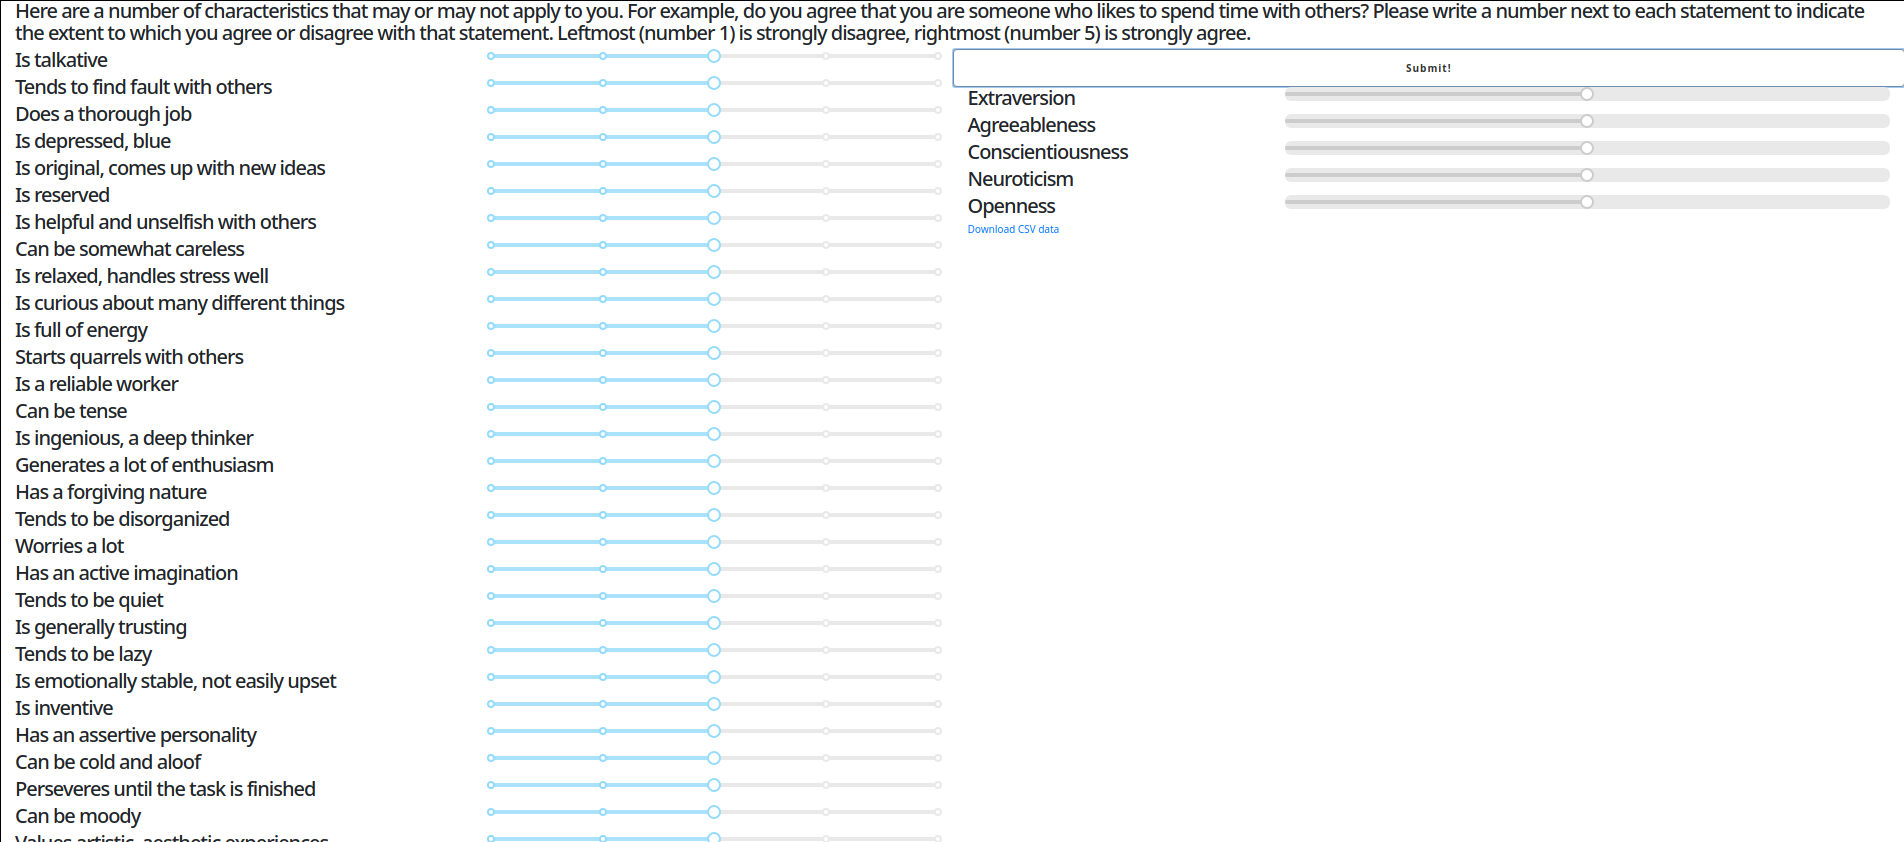
\includegraphics[width=\textwidth]{app}
\end{figure}
\chapter{Zaključak}

Ekspertni sustav za određivanje pet faktorskog modela ličnosti ima siru primjenu nego u psihometriji i kliničkom liječenju. Danas se često primjenjuje prilikom testova za posao radi sastavljanja balansiranih timova -- Otvoreni ljudi će željeti mijenjati stvari, savjesni i zatvoreni odražavati red, ugodni odrzadaju i potucu stabilnost i slogu tima te svaka osobina ličnosti ima svoje prednost, mane i komplementarne osobine. Cak i neurotičnost može biti korisna budući da averzija prema riziku izbjegava pretjeranu optimističnost i samozavaravanje.
Ovakav sustav pomaze svima uključenima brza, preciznije i standardizirano modeliranje raznolike ljudske ličnosti.

\bibliography{refs}
\bibliographystyle{fer}

\end{document}
